\section{A supervised model of dyadic sentiment}

\label{section:foreign_relations_supervised_model}

In the last chapter we described a model for identifying influential
documents.  A defining feature of that model was that it was
unsupervised; only after fitting the model could we compare the
inferred influence of an article with the number of citations it had
recieved.  In this section we will take a more direct approach,
fitting a model with labels \emph{defined} to represent the
information that we seek: whether there is a positive or negative
relationship between pairs of countries.

In outlining this model, we will discuss the two important assumptions
made in this paper: first, that there is a relationship between text
and the sentiment between pairs of countries; and second, that there
is a way to model the sentiment between countries by modeling
countries as vectors in a latent space.  After this we adjust the
model to extend it to the time-series domain.

\subsection{Inferring sentiment from text}
\label{section:text_regression}
The first key assumption that we make in this chapter is that when a
news source discusses the relationship between these nations, the
author's choice of words $\bm w_d \in \mathbb{N^+}^V$ reflects the
relationship between the countries.  This then means that we can
represent this relationship with a latent variable model.  Consider,
for example, the following passages (emphasis added by me):
\begin{itemize}
\item \begin{quote} ``In Government and opposition circles
      questions have swirled about how a \textbf{Palestinian} truck laden with
      explosives could have sailed past \textbf{Israeli} soldiers stationed at
      Gaza Strip checkpoints.  Some news reports said the vehicle had
      the required Israeli permits.'' \emph{Failed Truck-Bomb Plot Chills
      Israel-P.L.O. Autonomy Talks} \citep{nyt_haberman:1995}
  \end{quote}
\item \begin{quote} ``The leaders of \textbf{Egypt} and
    \textbf{Jordan} too have invested their prestige in the peace plan
    and would rejoice in private to see Islamic militants crushed.''
    \emph{Middle East Talks are Effort to Aid Peres and Arafat}
    \citep{nyt_jehl:1996}
    \end{quote}
\end{itemize}
In the first passage, Israel and Palestine have a tense relationship,
as suggested by the author's choice of the words ``explosives'',
``questions'', and even ``required''.  In the second passage, the
relationship---while not fabulous---is certainly more
positive, as suggested by words such as ``invested'', ``peace'', and
``rejoice''.

\paragraph{Paragraphs of text as a unit of analysis.} We will use
paragraphs of text which mention exactly two countries as the basic
unit of analysis in this chapter.\footnote{We provide more detail
  about tagging countries in the experiments section.}  Paragraphs of
text (like the two above) are small enough to contain simple ideas yet
large enough to discuss complete ideas---appropriate also for
discussing the relationship between pairs of countries.

We will model the relationship between text and sentiment with a
relatively simple model called text regression \citep{kogan:2009}.  In
text regression, we model sentiment using the wordcounts $\bm w_d$ of
each article:
\begin{align}
  s_d | \bm w_d, \bm \beta \sim \mathcal{N}( \bm w_d^T \bm \beta,
  \sigma_W^2 ) \nonumber \\
  \bm \beta \sim \mathcal{N}(0, \sigma_\beta^2 ).
  \label{eq:sentiment_text}
\end{align}
For the remainder of this section, we will assume that $\bm \beta$ is
observed, and therefore that the distribution of $s_d$ is a Gaussian with mean
$\bm w_d^T \bm \beta$.  We describe how to fit $\bm \beta$ with
\myeq{sentiment_text} and human labels in
Section~\ref{section:mturk}.

\subsection{Modeling interations with a latent space}
\label{sec:fr_latent_space_model}
The second important assumption we make in this chapter is that each
country can be described by a vector in some latent space, and that
the relationship between two countries is determined (up to
stochasticity) by the relationship between these countries' positions
in this latent space (this assumption is variously known as a latent
space assumption or multidimensional scaling).

We formalize the latent space assumption by letting each country $c$
take a position $\bm \bar x_{c,0} \in \mathbb{R}^p$ in a space of
latent political sentiment. As noted above, the sentiment of the
relationship between these two countries $c_1, c_2$ is described by
the scalar $s_{c_1,c_2} \in \mathbb{R}$.  During an interaction
between countries $c_1$ and $c_2$ which is described by document $d$,
we will assume that this interaction has sentiment $s_d$ between them.
This sentiment is determined by the interaction of their positions:
\begin{align}
  \bm x_{c_1,d} \sim \mathcal{N}(\bm \bar x_{c_1, 0}, \sigma_D^2) \nonumber \\
  \bm x_{c_2,d} \sim \mathcal{N}(\bm \bar x_{c_2, 0}, \sigma_D^2) \nonumber \\
  s_d := \mathcal{F}(\bm x_{c_1,d}, \bm x_{c_2,d}), \label{eq:sentiment_space}
\end{align}
for some suitable function $\mathcal{F}: \mathbb{R}^p \times \mathbb{R}^p
\rightarrow \mathbb{R}$ (see \mytab{fr_link_functions} for examples of
$\mathcal{F}$).  We have also introduced the auxiliary random
variables $x_{c_1}$ and $x_{c_2}$, which can be interpreted as
per-interaction positions.  We include them for algebraic convenience
which will be evident later.

\begin{figure}
  \center
\begin{tabular}{|l|l|m{3.9cm}|}
      \hline
      Description & $\mathcal{F}(\bm x_1, \bm x_2)$ & where ... \\
      \hline
      distance & $-\log(|| \bm z_{1} - \bm
      z_{2} ||_2^2 + 1)$ & $\bm z_{1} = \bm x_{1,2:D}, \bm z_2 = \bm x_{1,2:D}$ \\
      \hline
      inner product & $\bm z_{1}^T \bm z_{2}$ & $\bm z_{1} = \bm
      x_{1},$ $\bm z_2 = \bm x_{2}$ \\
      \hline
      intercept & $y_1 + y_2$ & $y_1 = x_{1,1}, y_2 = x_{2,1}$ \\
      \hline
      intercept/inner product & $y_1 + y_2 + \bm z_{1}^T \bm
     z_{2}$ & $y_1 = x_{1,1}, y_2 = x_{2,1},$ \\
    & & $\bm z_{1}
     = \bm x_{1,2:D}, \bm z_2 = \bm x_{2,2:D}$ \\
      \hline
     intercept/distance & $y_1 + y_2 - \log(|| \bm z_{1} - \bm
     z_{2} ||_2^2 + 1)$ & $y_1 = x_{1,1}, y_2 = x_{2,1},$ \\
     & & $\bm z_{1}
     = \bm x_{1,2:D}, \bm z_2 = \bm x_{2,2:D}$ \\
     \hline
    \end{tabular} \\
\label{fig:fr_link_functions}
\caption{Link functions $\mathcal{F}: \mathbb{R}^p \times \mathbb{R}^p
  \rightarrow \mathbb{R}$.  Intercept link functions introduce
  per-country intercepts that indicate how prone a country is to war;
  distance link functions are based on the distance between countries'
  vectors; and inner-product link functions represent sentiment as a
  function of countries' political ``orientations''.}
\end{figure}

If $\mathcal{F}$ is continuous and $c_1$ and $c_2$ are similar (as
measured by the distance between $\bm \bar x_{c_1}$ and $\bm \bar
x_{c_2}$), then $c_1$ and $c_2$ will interact with other countries in
similar ways.  Most importantly, by selecting $\mathcal{F}$
carefully, we can ensure that $\mathcal{F}(x_{c_1}, x_{c_2}) \ll 0$
indicates a poor relationship between $c_1$ and $c_2$, while
$\mathcal{F} \gg 0$ indicates a positive relationship.

A spatial a model provides us with two benefits. First, it provides
interpretability: we can summarize countries' relationships with other
countries succinctly with their positions $\bar x_c$.  Second, this
allows us to draw on existing work from multidimensional scaling,
which has been used successfully in both political science
\citep{martin:2002,jackman:2001} and social network modeling
\citep{hoff:2002,chang:2009}.

\subsection{A temporal model of interaction}
\label{sec:fr_time_series_model}
\begin{figure}
  \center
  \vspace{-55pt}
  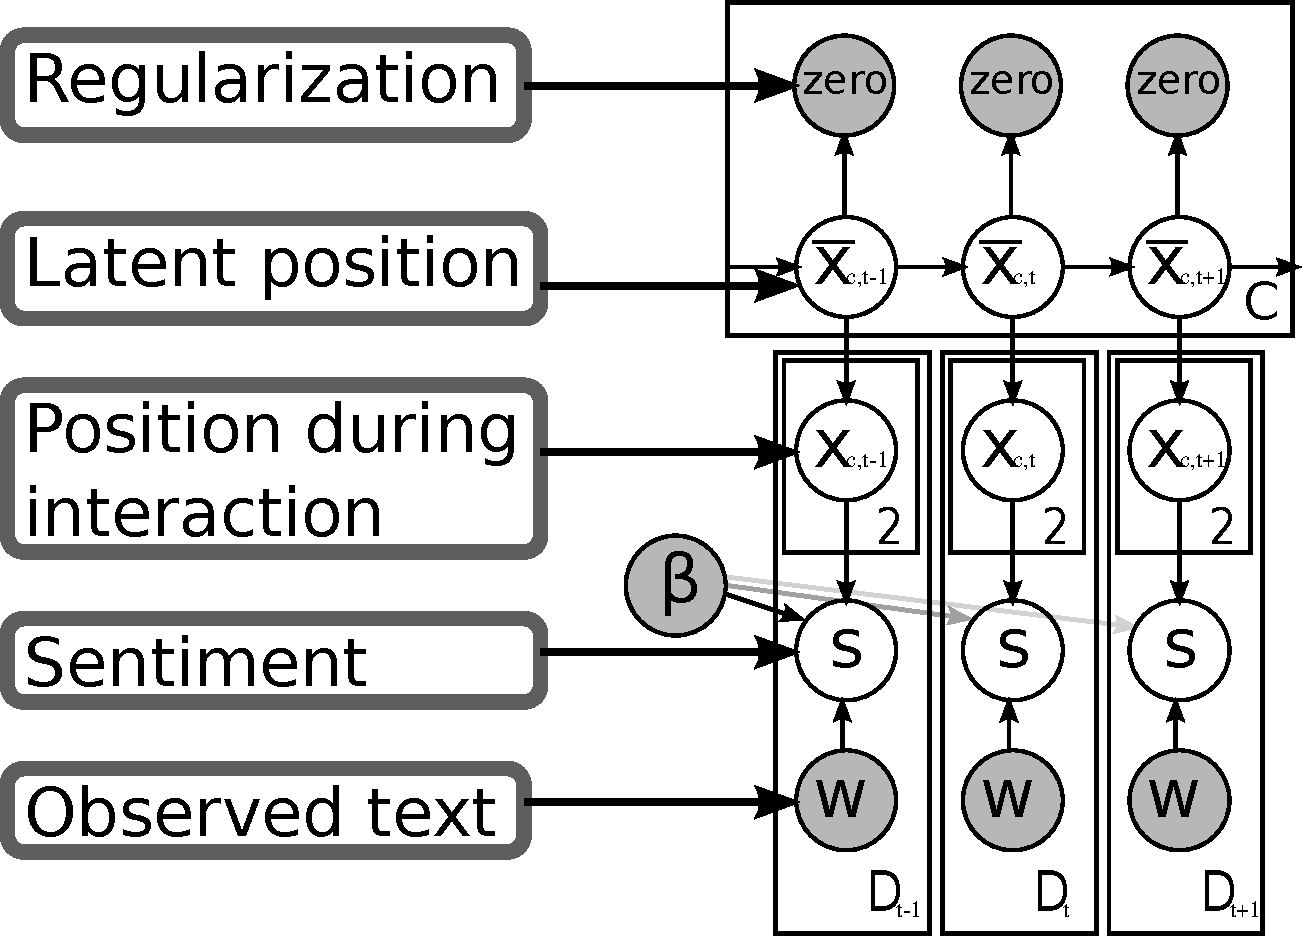
\includegraphics[width=0.5\textwidth]{chapter_foreign_relations/figures/countries_gm.pdf}
  \caption{A time-series model of countries' interactions.
    Pseudo-observations of ``zero'' are added for regularization.
    Amazon Mechanical Turk labels are used to fit $\bm \beta$, which is
    used to infer unobserved sentiments.}
  \label{fig:fa_gm}
\end{figure}

Foreign relations are not static; nations' alliances and preferences
change over time with the evolution of economies, technology, and
culture.  Therefore we make this a fully temporal model by
allowing each country's mean position $\bar x_{c,t}$ to drift over
time with the Markov transition
\begin{align}
  \label{eq:fr_interaction_position_given_mean}
  \bar x_{c,t} | \bar x_{c,t-1} \sim \mathcal{N}(\bar x_{c,t-1},
  \sigma_{\mbox{\tiny chain}}^2),
\end{align}
as shown in Figure~\ref{fig:fa_gm}. At any time $t$, we may observe
the relationship between states $c_1$ and $c_2$ in an article $d$.  As
before, the distribution of the sentiment between these countries is
entirely specified by their positions at this time:
\begin{align}
  x_{c_1,d} \sim \mathcal{N}(\bar x_{c_1, t}, \sigma_D^2) \nonumber \\
  x_{c_2,d} \sim \mathcal{N}(\bar x_{c_2, t}, \sigma_D^2) \nonumber \\
  s_d := \mathcal{F}(\bm x_{c_1,d}, \bm x_{c_2,d}), \label{eq:sentiment_space}
\end{align}
where we interpret $s_d$ as the sentiment between $c_1$ and $c_2$ as
reflected by article $d$ (which appeared at time $t_d$).

\paragraph{Regularization.} We add two additional notes to this mode
To complete this model, we add a standard normal prior to the ends of
the chain (i.e., $p(\bm \bar x_{c, 0}) = p(\bm \bar x_{c,T}) =
\mathcal{N}(0, 1)$ for all countries $c$).  We also add an additional
regularization term which we call zero-reversion.  This term manifests
itself as observations $p(x | \bm \bar x_{c, t}) = \mathcal{N}(0,
\sigma_{\mbox{\tiny zero}}^2)$ for all times $t = 0, \ldots, T$ and
all countries $c$.  The role of this regularization term is to enable .

For the purposes of countries' positions in the latent-space model,
however, we will use the symmetry of the Gaussian to model text as if
it were conditioned on sentiment: $p(s_d | \bm w_d^T \bm \beta,
\sigma_W^2) = p( \bm w_d^T \bm \beta | s_d, \sigma_W^2 )$.  This
allows us to reconcile \myeq{sentiment_text} and
\myeq{sentiment_space}, so that the distribution of sentiment
conditioned on text and countries' positions is:
\begin{align}
  p(s_d | \bm w_d, \bm \beta, x_{c_1,d}, x_{c_2,d}) & \propto
  p(\bm w_d^T \bm \beta | s_d, \sigma_W^2 )
  p(x_{c_1,d} | \bar x_{c_1, t}, \sigma_D^2)
  p(x_{c_2,d} | \bar x_{c_2, t}, \sigma_D^2) \nonumber \\
  & \hspace{20pt} \mbox{ such that } s_d = \mathcal{F}(x_{c_1,t},
  x_{c_2,t}) \nonumber \\
  & = 
  p(\bm w_d^T \bm \beta |
    \mathcal{F}(x_{c_1,t}, x_{c_2,t}), \sigma_W^2 )
  p(x_{c_1,d} | \bar x_{c_1, t}, \sigma_D^2)
  p(x_{c_2,d} | \bar x_{c_2, t}, \sigma_D^2).
\end{align}

% In addition, a UN resolution may come up for vote at any time.  States
% cast a vote based on their current positions:
% \begin{align}
% x_{c_1,d} \sim N(\bar x_{c_1, t}, \sigma_D^2) \nonumber \\
% p(v_{cr}) = \sigma(x_{c_2, t} b_r + a_r) \nonumber \\
% \end{align}

% \begin{wrapfigure}{r}{0.4\textwidth}
%   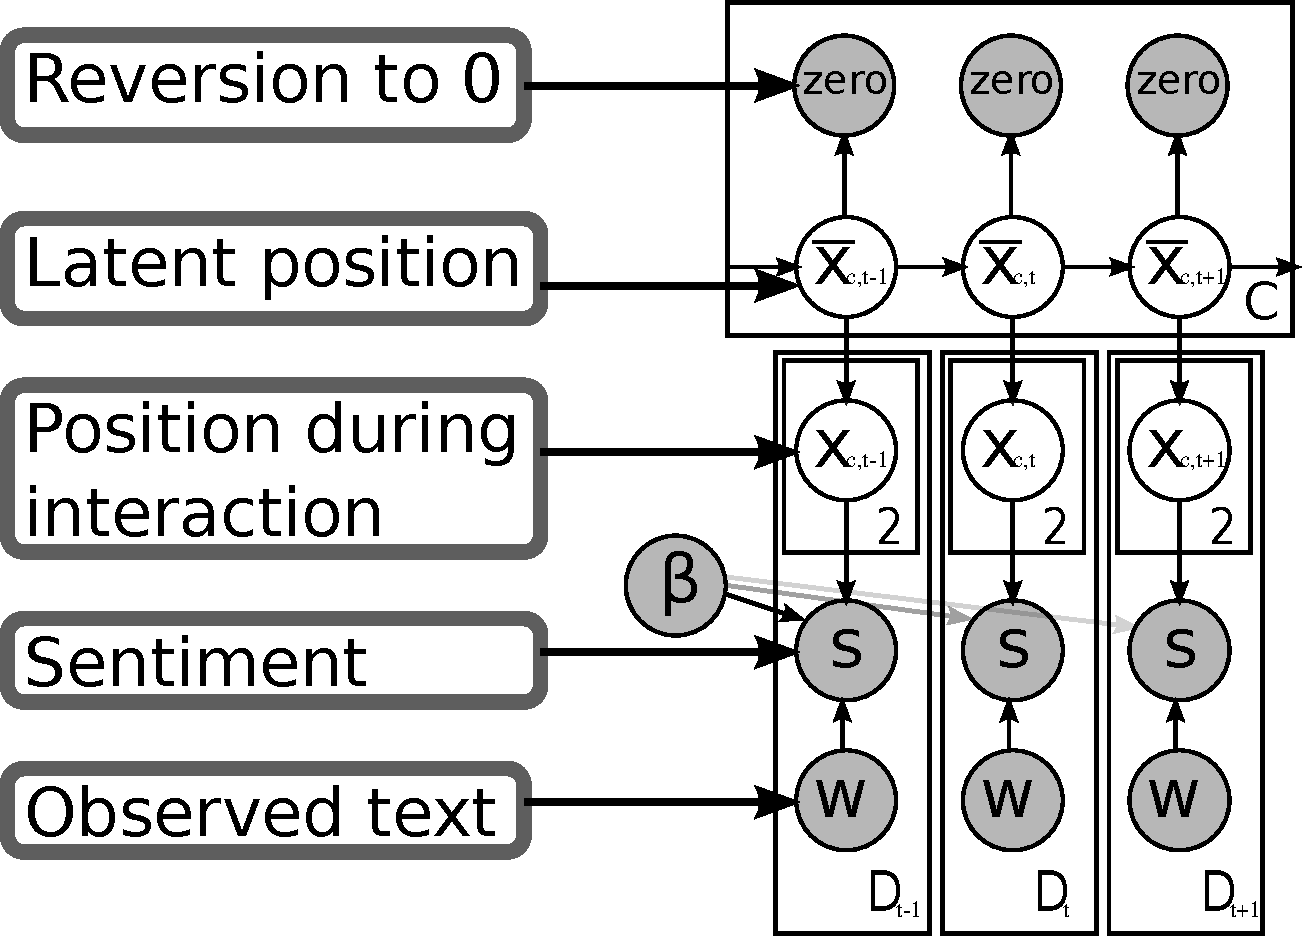
\includegraphics[width=0.4\textwidth]{figs/countries_gm.pdf}
%   \caption{The full time-series model of interaction by countries.
%     The large plate shows replication of a Markov chain for each
%     country.  Certain countries interact at each epoch -- possibly
%     multiple times -- with sentiment $s$.}
%   \label{fig:countries_by_ip}
% \end{wrapfigure}

\paragraph{A brief comment on notation.} Before proceeding to
inference and the experimental validation of this model, we pause to
summarize our use of notation.  In this chapter, we will use notation
flexibly when it is convenient.  The typical unit of discussion will
be the $d$th document occurring at time $t$.  The $d$th document
discusses two countries, $c_1$ and $c_2$; these define a tuple $(\{
c_1, c_2 \}, d, t)$ (where the set $\{ c_1, c_2 \} = \{ c_2, c_1 \}$).
We will generally use $d$ to index documents, $t$ to index time, and
$c$ to index a country.  When document $d$ is given, we may refer to
its time as $t_d$ (which is unique) or to the two interacting
countries as $c_{d,1},c_{d,2}$ or $c_1,c_2$.  Alternatively, we may
refer to the documents in which a country $c$ appears as $d_{c,1},
\ldots, d_{c,D}$.  As another example, we may describe a country's
position $x_{(c_1,d,t)}$ variously as $x_{c_{d,1}}$, $x_{d,1}$, or even $x_c$
if the context is clear. Finally, the sentiment between two countries
might be variously described as $s_d$, $s_{c_1,c_2}$, $s_{d,t}$, or
$s_{c_1,c_2,d,t}$.

\subsection{Related work}

The field of sentiment analysis has received considerable attention in
the last couple of decades and is used in a variety of industry
fields, ranging from automated trading strategies to restaurant
recommendation sites.  Models in which individual words are assigned a
weight are common; see \cite{pang:2008} provide a review of recent
developments in this field.  See \cite{taddy:2012} for a model which
uses inverse regression on wordcounts for results which compare
favorably with alternatives.

% Democracy, Political Similarity, and International Alliances, 1816-1992
% Brian Lai
% Dan Reiterb
% Department of Political Science, Emory University
Spatial models such as Item Response Theory (IRT) have been developed
over the past century by quantitative social scientists for analyzing
behavior.  While much of this work has been used to model
parliamentary voting behavior, these techniques have also been used to
model voting in the UN General Assembly. Gartzke et al., for example,
use these votes and alliance models to study the nations' affinities
\citep{gartzke:1998}.

These models have been developed for dyadic data more fully in network
models such as the latent space model \citep{hoff:2002,sarkar:2005}, in
which the probability of a link between two nodes is a function of
their latent-space distance.  The qualitative relationship of
entities' dyadic relationships has been more fully developed with text
by the relational topic model, which uses free text to model the
relationship between actors in an unsupervised setting
\citep{chang:2009}.

The areas of sentiment analysis and dyadic models have been combined
in recent work focused on content recommendation and unsupervised
network discovery.  Recommendation systems have been specialized to
items with text for recommmending content such as Web content
\citep{agarwal:2010} and academic journals \citep{wang:2011}; both of
these applications used latent Dirichlet allocation for modeling text.
\cite{chang:2009} has also used unsupervised topic models to discover
relationships between entities.
% Supervised topic models


% Affinity of states dataset: 
% Fading Friendships (working paper)
% Alliances, Affinities and the Activation of International Identities∗
% Erik Gartzke†
% Alex Weisiger‡
% 7 March 2011

\subsection{Inference}
\label{sec:fr_inference}
We fit the \emph{MAP} objective of this probabilistic model.  This has
the benefit of both clean exposition and simple implementation, and it
can be interpreted as a form of unregularized variational inference.
We optimize the \emph{MAP} objective in this model using an
expectation maximization (EM) algorithm, which is simplified because
we have designed the probabilistic objective to make inference
particularly manageable.

\subsubsection{An expectation maximization algorithm}
The MAP solution to this problem corresponds to an
expectation-maximization (EM) algorithm because of the way we have
specified $p(x_{c,d} | \bm \bar x_{c, t_d})$.  This makes inference
much simpler and allows us to take advantage of a Kalman smoother.
Instead of optimizing each variable in the objective, we alternate
between optimizing the variables $x_{c,d,t}, s_d$ in an E step and the
variable $\bm \bar x_{c,t}$ in the M step.

% To motivate and derive this M step, we will
% optimize the following lower bound on the data likelihood:
% \begin{align}
%   \mathcal{L}_x = \log p(s_d, \bm w, \bm \beta, x)
%   % & \propto p(s_d | \bm w, \beta, x, \bm \beta) \\
%   & = \log \expectq{ \int_{\bar \bm z} \frac{q(\bar x)}{q(\bar x)}
%     p(s_d | \bm w, \bm \beta, x, \bar \bm z) dz } \nonumber \\
%   & \ge \expectq{ q(\bar x)
%     \log \frac{ p(s_d | \bm w, \bm \beta, x) }{
%       q(\bar x)} } \\
%   & = \expectq{ \log p(s_d | \bm w, \bm \beta, x) }
%     - H(q(\bm \bar x)), \\
% \end{align}
% where $H(q)$ is the entropy of the expectation distribution $q =
% \expect{\bm \bar x}$.

% Notice that this is exactly the same form as the variational
% objective; making a point estimate of $\expect{\bar \bm x}$ results in
% a degenerate entropy, leaving us with the original objective 

\paragraph{M Step.} In the M step, we seek to estimate the mean
$\expect{\bm \bar x_{c,t}} | x, \beta, s$ of each country $c$'s
position.  Because the Markov blanket of each variable $\bm \bar
x_{c,t}$ is specified by Gaussian distributions, we have that, at the
optimum,
\begin{align}
\bm \bar x | x, \beta, s = \expect{x} | x, \beta, s
  = \underset{\bm \bar x} { \arg \max }\hspace{3pt} p(s, x, \beta, \bm \bar x),
\end{align}
which means that finding the optimal value of $\bm \bar x | s, x,
\beta$ is equivalent to estimating this expectation of $x_t$.  We can
estimate $\bm \bar x | s, x, \beta = \expect{x} | x, s, \beta$ using a
modified Kalman smoother \cite{kalman:1960}.  This step differs from a
standard Kalman smoother in that we have no observations $x | \bm \bar
x$ on some dates and multiple observations $x | \bm \bar x$ on other
dates.

\paragraph{Kalman updates.} As with a standard Kalman smoother, the
modified Kalman smoother requires a forward filter step and a backward
filter step.  The forward filter estimates the mean position given all
previous observations:
\begin{align}
  \bar x_{\mbox{\tiny forth},c,t} | \bar x_{\mbox{\tiny forth},c,t-1},
  \{ x_{c,d,t-1} \}_{d} =
  & \gets \frac{\bar x_{\mbox{\tiny forth},c,t-1} / \sigma_{\mbox{\tiny forth},t-1}^2
    + \sum_{d=1}^{D_{c,t-1}} x_{c,d,t-1} / \sigma_{\mbox{\tiny obs}}^2}
  {1 / \sigma_{\mbox{\tiny forth},t-1}^2 + 1 / \sigma_{\mbox{\tiny obs}}^2} \\
  \sigma_{\mbox{\tiny forth},t}^2
  & \gets \frac{1}{1 / \sigma_{\mbox{\tiny forth},t - 1}^2
    + D_{c,t-1} / \sigma_{\mbox{\tiny obs}}^2} + \sigma_{\mbox{\tiny chain}}^2,
\end{align}
where we have used $x_{c,d,t}$ to describe the position of country $c$
at time $t$ for interaction $d$ and there are $D_{ct}$ documents at
time $t$ discussing country $c$.  We also use initial condition $\bar
x_{c,0} = 0, \sigma_{\mbox{\tiny forth},0}^2=10$.  The backward step
estimates the chain's mean given all current and future observations:
\begin{align}
  \bar x_{\mbox{\tiny back},c,t} | \bar x_{\mbox{\tiny back,c,t+1}}, \{ x_{c,d,t} \}_d
  & \gets \frac{\bar x_{\mbox{\tiny back},c,t+1} / \sigma_{t+1}^2
    + \sum_{d=1}^{D_{c,t}} x_{c,d,t} / \sigma_{\mbox{\tiny obs}}^2}
  {1 / \sigma_{\mbox{\tiny back},t-1}^2 + 1 / \sigma_{\mbox{\tiny obs}}^2} \nonumber \\
  \sigma_{\mbox{\tiny back},t}^2
  & \gets \frac{1}{1 / (\sigma_{\mbox{\tiny back},t + 1}^2 + \sigma_{\mbox{\tiny chain}}^2)
    + D_{c,t} / \sigma_{\tiny obs}^2},
\end{align}
with initial conditions $\bar x_{\mbox{\tiny back},c,T} = 0,
\sigma_{\mbox{\tiny backward},T}^2=10$. The smoothed means---that is,
the mean of countries' positions at time $t$ given observations before
and after $t$---are
\begin{align}
  \bm \bar x_{c,t} | x_{c,t} & = \expect{ x_{c,t}} | \bar x_{\mbox{\tiny forth,c,t}}, \bar x_{\mbox{\tiny back,c,t}}, \sigma_{\mbox{\tiny back}}^2, \sigma_{\mbox{\tiny forth}}^2 \nonumber \\
  & = \frac{\bar x_{\mbox{\tiny forth},c,t} / \sigma_{\mbox{\tiny forth},t}^2
    + \bar x_{\mbox{\tiny back},c,t} / \sigma_{\mbox{\tiny back},t}^2}
  {1 / \sigma_{\mbox{\tiny forth},t}^2
    + 1 / \sigma_{\mbox{\tiny back},t}^2}
\end{align}

% x_{c,d,t}
\paragraph{E Step.} In the E-step, our goal is to infer each nation's
position $x_{c_{d,1}} | \bm \bar{x}_{c,d,t}, x_{c_{d,2}}, s_d, \bm
w_d$ during interaction $d$ given its expected mean $\bm \bar
x_{c_{d,1},t_d}$ and the text $\bm w_d$ describing this interaction,
\emph{and} given the other country's position for this interaction.
Assuming that this country is indexed by $c_1$ in each document, we
find these positions by gradient ascent on each interaction:
\begin{align}
  x_{c_{d, 1}, t} & \gets \underset{ x }
  {\arg \max}\hspace{3pt}
  p(\bm w_d^T \bm \beta | \mathcal{F}(x, x_{c_{d,2},t}),
  \bm \bar x_{c_{d,1},t} ) \nonumber \\
  & = \underset{x}
  { \arg \max }\hspace{3pt}
  p(\bm w_d^T \bm \beta | \mathcal{F}(x, x_{c_{d,2},t}),
  \bm \beta)
  p(x | \bar x_{c_{d,1},t} ),
\end{align}
where the last term is given by the distribution
\myeq{fr_interaction_position_given_mean}.  For convenience, we
iterate between updating $x_{\{c,\cdot\}}$ for all interactions
involving country $c$ and updating $\bm \bar x_{c,t}$ with the M step
for all times $t$.

\subsection{Empirical studies: comparisons with ground truth}
We now turn to an experimental analysis of this model.  Our goal in
this analysis is to demonstrate first that the model captures
statistically meaningful patterns in a time-series collection of
newspaper documents and second that it can provide a meaningful view
into countries' relationships with one another.

We first describe the two label types we have used to define sentiment $s_d$
within this model and the newspaper archive to which we fit this
model.  We then evaluate the model's ability to infer the
relationships between countries and compare results from models
inferred with the two different label types.

\subsection{Parsing the New York Times}

We fit and evaluate this model over news articles discussing 245
nations and territories from twenty years of the \emph{New York Times}
(NYT).  This collection spanned the years 1987 to 2007, a period which
included both the Persian Gulf and Iraq wars; the collapse of the
Soviet Union; the reunification of Germany; September 11th, 2001; and
countless other world events.

\paragraph{Data preparation.}
We used articles from the Foreign, Business, Financial, and Magazine
desks of the newspaper during this period. As noted in
\mysec{text_regression}, we split this collection into paragraphs
defined by Times editors and used the subset of paragraphs which
discuss exactly two nations as ``documents'' $d$.  This resulted in
257,472 paragraphs.  We then defined a vocabulary to be those words
which satisfied three criteria:
\begin{itemize}
  \item Appeared at least twenty times,
  \item Appeared in no more than 40\% of documents, and
  \item Appeared in at least 0.1\% of documents.
\end{itemize}

This resulted in a vocabulary of 5,958 words, mentioned in 40,356
paragraphs. We randomly selected 80\% (32,249) distinct paragraphs
from this set as training examples and used the remaining examples to
evaluate our model.

\subsection{Coding sentiment}
\label{section:sentiment_models}

We next estimated $\bm \beta$ by fitting ridge regression on a subset
of the training examples.  We labeled training examples with
information from both inexperienced ``workers'' and ``expert labels'',
representing vastly different ends of the label spectrum (as we will
see, they result in strikingly similar results).

\subsubsection{Novice labels: Amazon Mechanical Turk ratings}
\label{section:mturk}

\emph{Amazon Mechanical Turk} (AMT) is a crowdsourcing platform which
provides a \emph{requestor} (the author of this thesis) with access to
thousands of \emph{workers} who perform simple tasks over the
Internet.  Although the requestor can use tests to ensure that workers
are high-quality, as well as reject the work of low-quality workers,
these workers are typically not experts.

\begin{figure*}
  \setlength\fboxsep{0pt}
  \setlength\fboxrule{0.5pt}
  \center \fbox{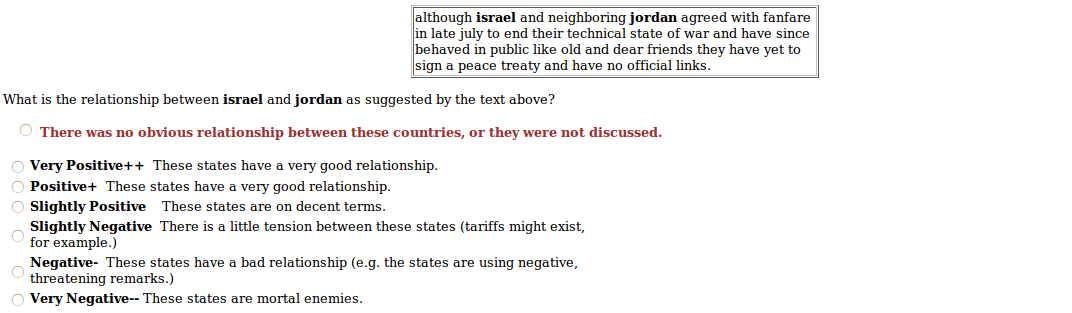
\includegraphics[width=1.0\textwidth]{chapter_foreign_relations/figures/mturk_screenshot.png}}
  \label{fig:mechanical_turk_sample}
  \small\caption{A screenshot of a Mechanical Turk labeling task.
    Sometimes relationships may be complicated; both raters gave this
    example a score of ``slightly positive''.}
  \normalsize
\end{figure*}

To fit the model, we asked \emph{Amazon Mechanical Turk} workers to
rate the sentiment between two nations mentioned in the text of a
paragraph on the scale -5 (mortal enemies), $\ldots$, 5 (very good
relationship). We illustrate a rating task (as seen by a Mechanical
Turk worker) in \myfig{mechanical_turk_sample}. Raters were asked to
review a random subset of 3607 paragraphs like this from the original
collection.  Before fitting the model, we manually disqualified eight
raters (out of 85) who consistently performed poor ratings.

With all rated paragraphs which were not in the test set, we fit the
coefficients $\bm \beta$ of the text regression discussed in
Section~\ref{section:model}.  This coefficient was then treated as
constant in the joint model in Figure~\ref{fig:fa_gm} to allow us to
infer sentiment from the words of all 32,249 training paragraphs.
This resulted in a regression weight $\beta_w$ for each word $w$,
which we illustrate in \myfig{fr_example_betas} (left).

\subsubsection{Expert labels: Correlates of War}
\label{section:correlates_of_war}

We also used a combined set of expert labels based on the Correlates
of War \citep{sarkees:2010} and Issue Correlates of War
\citep{hensel:2001}.
\begin{itemize}
  \item The \emph{Correlates of War} project ``seeks to facilitate the
    collection, dissemination, and use of accurate and reliable
    quantitative data in international relations''
    \citep{cow_webpage:2012}.  The project provides labels describing the
    relationships between pairs of countries from 1823 to 2003.
    At-war is a binary relationship (either countries are at war, or
    they are at peace). We used a list of CoW inter-state wars
    (version 4.0) from 1823 to 2003
    \citep{sarkees:2010}.
  \item The \emph{Issue Correlates of War} project ``is a research
    project that is collecting systematic data on contentious issues
    in world politics'' \citep{icow_webpage:2012}, and they provide
    expert labels on a variety of inter-state conflicts that \emph{do
      not require militarized conflict}.  However, these issue label
    do require documented evidence of contention between states; such
    issues include maritime and territorial disputes
    \citep{icow_webpage:2012,hensel:2001}. The Issue Correlates of War
    are not part of the same project (or produced by the same
    researchers) as the Correlates of War.
\end{itemize}

We combined the datasets by treating two countries as having a rating
of -5 if they are at war at the time an article was written in the
Correlates of War codes and -1 if there was any contentious issue
between the countries in the Issue Correlates of War.  All other pairs
of countries were treated as having a rating of 0.1.  These values are
somewhat arbitrary (we could have chosen -6.3 for a bad relationship),
but they were selected to correspond roughly to the range of the
Mechanical Turk labels.  Further, they were selected once and kept
fixed---changing them during analysis could compromise the statistical
power of the results below.

As before, we fit the text regression parameters $\bm \beta$ using
these labels on the training set and evaluated countries' ratings on
the test dataset. We illustrate the coefficient $\bm \beta$ fit to
CoW-labeled paragraphs in \myfig{fr_example_betas} (left).

\begin{figure}
  \begin{tabular}{cc}
    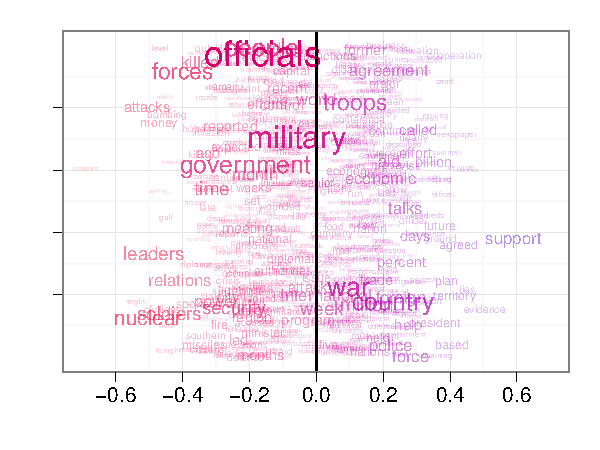
\includegraphics[width=0.4\textwidth]{chapter_foreign_relations/figures/mturk_sample_words.pdf} &
    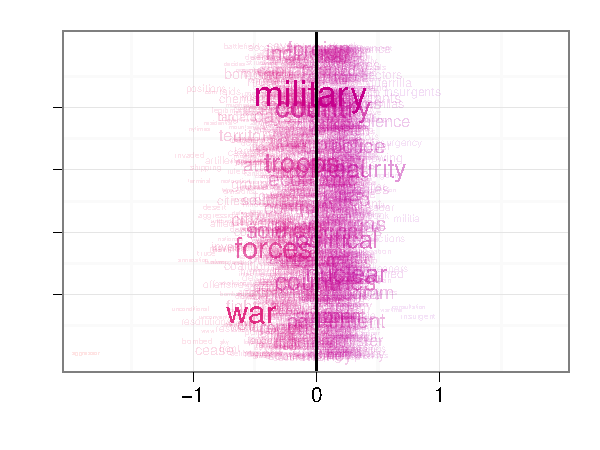
\includegraphics[width=0.4\textwidth]{chapter_foreign_relations/figures/cow_sample_words.pdf} \\
    \end{tabular}
  \caption{Coefficients $\bm \beta_w$ for selected words $w$ fit on text
    labeled by Amazon Mechanical Turk workers (left) and Correlates of
    War data (right). Coefficients fit from Mechanical Turk labels are
    more clearly separated than those fit to Correlates of War labels;
    this is likely due to explicit positive sentiment in that dataset.
    The $x$-axis is $\bm \beta$, and the $y$-axis is used for display (it
    corresponds to no variable).  Size of each word is proportional to
    $\sqrt{\mbox{frequency}}$, and color corresponds to $\bm \beta$.}
  \label{fig:fr_example_betas}
\end{figure}

\subsubsection{Casual vs. expert labels}
The CoW represent a data source which is modestly related to
Mechanical Turk ratings. In the NYT dataset, CoW ratings and
Mechanical Turk ratings were correlated at $\sigma=0.196$.  We can
better understand the difference between these ratings with some
examples of paragraphs $d$ having high and low inter-country sentiment
$s_d$:
\begin{itemize}
  \item AMT $= 1$, CoW $=-5$: \begin{quote} \emph{As an
    indication of the dangers the damage occurred in waters where
    military spokesmen said no mines had been suspected before but
    where a \textbf{Saudi} officer said today that some 22 were later
    found. \textbf{Iraq}i mines widely deployed [sic]} (February 1991)
    \citep{cushman:1991}
\end{quote}
  \item AMT $ = -5$, CoW $=0.1$: \begin{quote}\emph{Not since
    the grim old days of the cold war have relations between the
    \textbf{United States} and \textbf{Russia} been quite as problematic as they
    are this weekend on the eve of president clinton's visit for
    celebrations marking the 50th anniversary of the allied victory in
    europe in World War II.} (May 1995) \citep{apple:1995}
\end{quote}
\end{itemize}

The first of these examples outlines a limitation in our modeling
assumptions: a single paragraph is sometimes too small a unit of
discussion.  In this example, Mechanical Turk workers likely missed
the larger context of the article about the Gulf war (including the
article's title, \emph{War in the Gulf: Sea Mines; Allied Ships Hunt
  Gulf for Iraqi Mines}).

The second example represents a limitation of both data sources.  The
two Mechanical Turk ratings of -5 were clearly too strong, as the
countries are not at war; but AMT workers likely based their rating in
part on the reference to World War II (the instructions provided to
MTurk workers suggest that a rating of -3 or -1 would have been more
appropriate).  In 1995, the United States and Russia were not at war
and had no documented territorial conflicts.  This means that this
sentiment was not reflected in the CoW labels -- which defaulted to
0.1.

\label{section:experiments}

\subsection{Quantitative results}

\begin{figure}
%%   \begin{tabular}{|c|c|c|c|c|c|c|c|}
%%    \hline
%%   Link $\mathcal{F}(\bm x_{c_1}, y_{c_1}, \bm x_{c_2}, y_{c_2})$ & & & & & & \\
%%   \hline
%%   \textbf{Dimension of $\bm x$} & 0 & 1 & 2 & 3 & 4 & 5 & 6 & 7 & 8 & 9 \\
%%   \hline
%%   $y_{c_1} + y_{c_2}$ & 0.0964 & - & - & - & - & - & - & - & - & - \\
%%   \hline
%%   $\bm x_{c_1}^T \bm x_{c_2}$
%%   & 0.1036 & 0.1013 & 0.1050 & 0.1038 & 0.1033 & 0.1025 & 0.1018 & & & \\
%%   \hline
%%   $y_{c_1} + y_{c_2} + \bm x_{c_1}^T \bm x_{c_2}$
%%   & 0.0964 & 0.0943 & 0.0940 & 0.0936 & 0.0935 & 0.0934 & 0.0934 & & & \\
%%   \hline
%%   $-\log(||\bm x_{c_1} - \bm x_{c_2}||_2^2 + 1)$
%%   & 0.1036 & 0.1037 & 0.0978 & 0.0957 & 0.0951 & 0.0947 & 0.0943 & & & \\
%%   \hline
%%   $y_{c_1} + y_{c_2} -\log(||\bm x_{c_1} - \bm x_{c_2}||_2^2 + 1)$
%%   & 0.0964 & 0.0949 & 0.0943 & 0.0938 & 0.0939 & 0.0937 & 0.0936 & & & \\
%%   \hline
%%   mean($\{s_d\}_d$) & 0.1036 & - & - & - & - & - & - & & & \\
%%   \hline
%%   \end{tabular}
%%   \vspace{30pt}
%%   \begin{tabular}{|c|c|c|c|c|c|c|c|}
%%    \hline
%%   Link $\mathcal{F}(\bm x_{c_1}, y_{c_1}, \bm x_{c_2}, y_{c_2})$ & & & \\
%%   \hline
%%   \textbf{Dimension of $\bm x$} & 0 & 1 & 2 & 3 & 4 & 5 & 6 \\
%%   \hline
%%   $y_{c_1} + y_{c_2}$ & 0.0964 & - & - & - & - & - & - \\
%%   \hline
%%   $\bm x_{c_1}^T \bm x_{c_2}$
%%   & 0.1036 & 0.1013 & 0.1050 & 0.1038 & 0.1033 & 0.1025 & 0.1018 \\
%%   \hline
%%   $y_{c_1} + y_{c_2} + \bm x_{c_1}^T \bm x_{c_2}$
%%   & 0.0964 & 0.0943 & 0.0940 & 0.0936 & 0.0935 & 0.0934 & 0.0934 \\
%%   \hline
%%   $-\log(||\bm x_{c_1} - \bm x_{c_2}||_2^2 + 1)$
%%   & 0.1036 & 0.1037 & 0.0978 & 0.0957 & 0.0951 & 0.0947 & 0.0943 \\
%%   \hline
%%   $y_{c_1} + y_{c_2} -\log(||\bm x_{c_1} - \bm x_{c_2}||_2^2 + 1)$
%%   & 0.0964 & 0.0949 & 0.0943 & 0.0938 & 0.0939 & 0.0937 & 0.0936 \\
%%   \hline
%%   mean($\{s_d\}_d$) & 0.1036 & - & - & - & - & - & - \\
%%   \hline
\begin{tabular}{|c|c|c|}
\hline
  \begin{minipage}{2cm}  \vspace{-3cm} \textbf{Correlates} \\ \textbf{of War}
    \vspace{4cm} \end{minipage}
  & 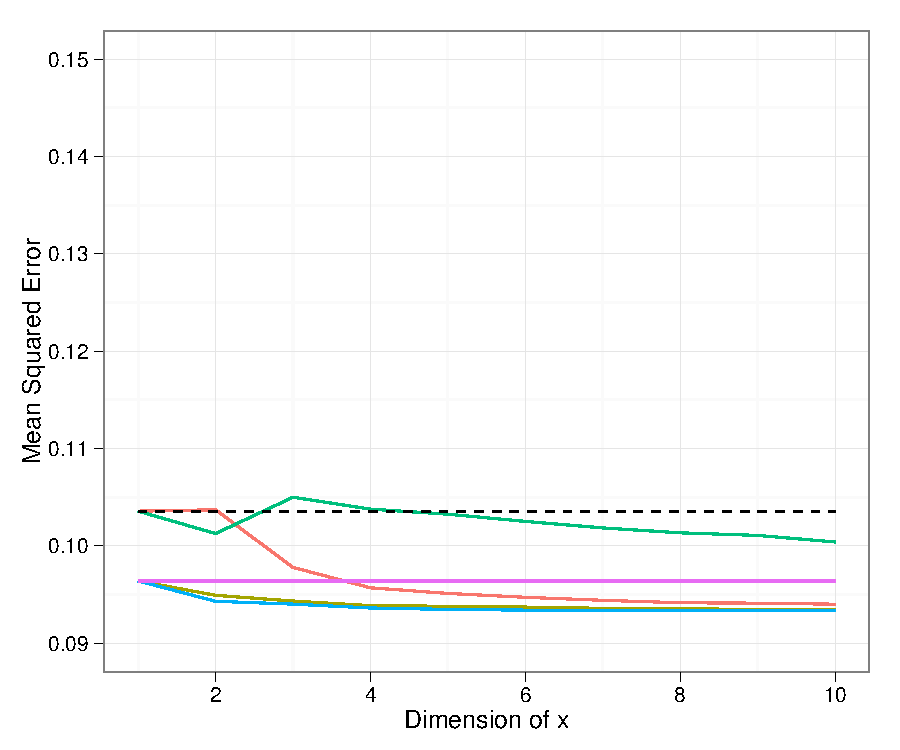
\includegraphics[height=0.27\textheight]{chapter_foreign_relations/figures/008_static_model_results.pdf}
  & 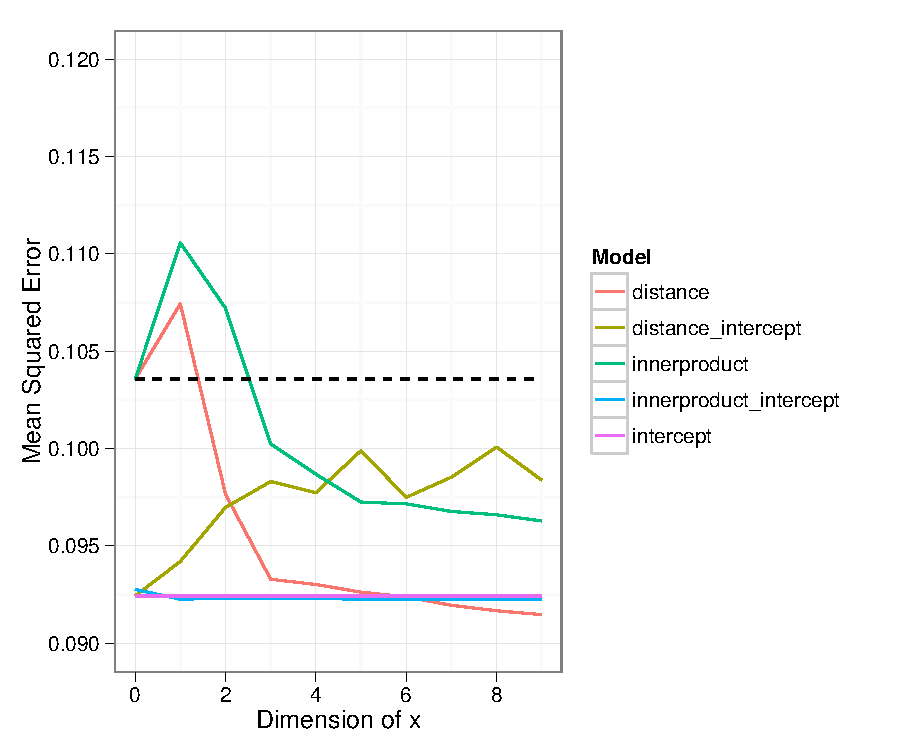
\includegraphics[height=0.27\textheight]{chapter_foreign_relations/figures/009_dynamic_model_results.pdf}
  \\
\hline
  \begin{minipage}{2cm} \vspace{-7cm} \textbf{Mechanical} \\
    \textbf{Turk} \end{minipage}
  & 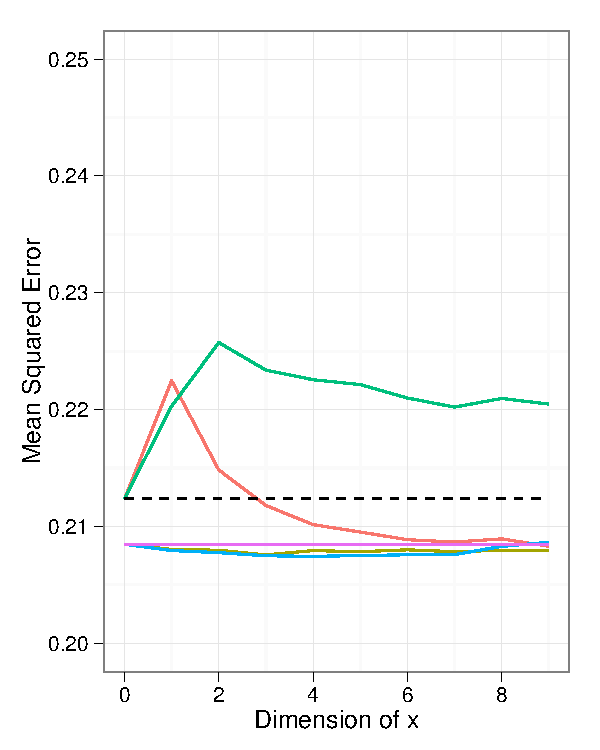
\includegraphics[height=0.27\textheight]{chapter_foreign_relations/figures/010_static_model_results.pdf}
  & 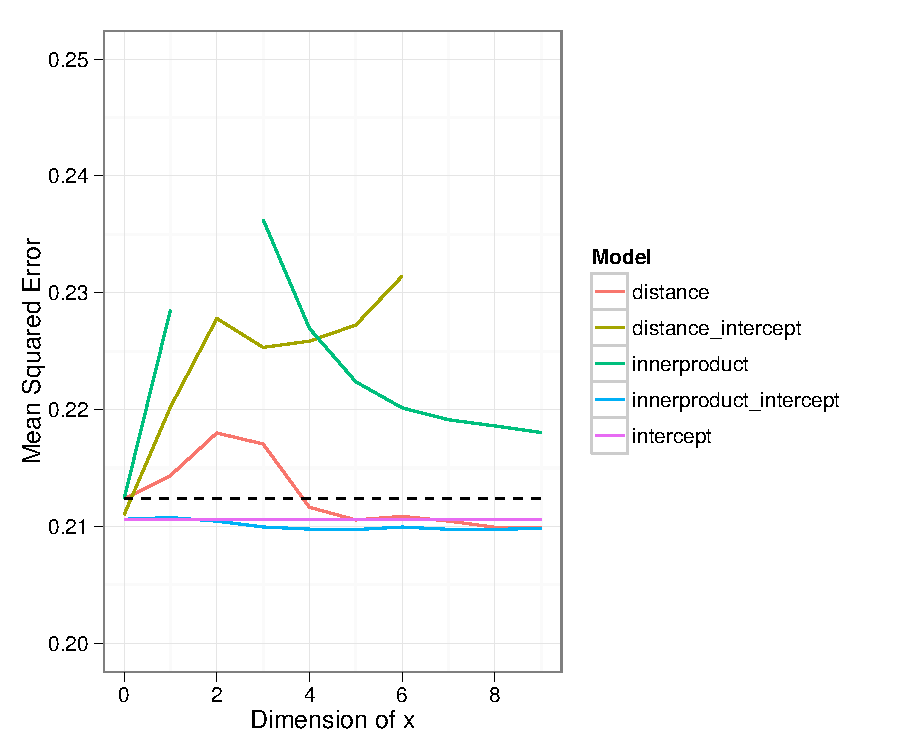
\includegraphics[height=0.27\textheight]{chapter_foreign_relations/figures/010_dynamic_model_results.pdf}
  \\
\hline
 & \textbf{Static} & \textbf{Dynamic (interaction over time)} \\
\hline
\end{tabular}
  \label{fig:fr_supervised_performance}
   \caption{The dyadic sentiment model captures text well . Each
     colored line represents performance of the supervised model on a collection
     of heldout documents across twenty years of New York Times
     articles. An inner-product model with four dimensions (plus
     intercepts) performs well for most settings.  A distance model
     with many dimensions but no intercepts also performs well across
     a range of assumptions, performing best with many dimensions.}
\end{figure}

\subsubsection{Inference and Prediction}
We next turn to an empirical validation of the model laid out so far
chapter. After fitting $\bm \beta$ to each set of labels on a subset
of training documents, we estimated the MAP solution $\bm \bar x, x, s
| \bm \beta, \bm w$ using the entire training set as set forth in
\mysec{fr_inference}.

For two nations $c_1$ and $c_2$ mentioned together at time $t$, we
predict their sentiment to be $\tilde s_{c_1, c_2} = \bar x_{c_1,t}
\bar x_{c_2, t}$ and calculate the mean-squared error between that
prediction and their predicted sentiment $\bm \beta^T \bm w_d$ under
text regression.

We made the latter choice so we could analyze the text regression part
of the model separately from the latent-space assumption (analyzing
them together would make it difficult to discern the effect of each
model).

\paragraph{Text regression.} The text-regression model for CoW labels
predicted heldout labels with MSE $0.98$, compared with $1.02$ if we
estimate using the empirical mean $\bar s=-0.21$ of training
examles. The text-regression model for AMT predicted heldout labels
with MSE of $6.37$, compared with $6.78$ under the empirical mean.  We
ignored words 

While these errors are very large compared to the variance of the
sentiment label, the scale of these errors is a result of the small
number of training examples, the large number of features (1998 in
each case, and the sparsity of these features).  Still, we find that
the coefficients $\bm \beta_{\mbox{\tiny CoW}}, \bm \beta_{\mbox{\tiny
    AMT}}$ learned from the respective CoW and AMT labels are
subjectively meaningful.  We illustrate the coefficients fit with
these labels in \myfig{fr_example_betas}.  The coefficients $\bm
\beta_{\mbox{\tiny CoW}}$ and $\bm \beta_{\mbox{\tiny AMT}}$ are
correlated at $\sigma=0.18$.

\paragraph{Static latent space.}
With the text model in place, we next turn to evaluating the
latent-space assumption.  To do this, we hold fixed the coefficients
$\bm \beta_{\mbox{\tiny CoW}}, \bm \beta_{\mbox{\tiny AMT}}$.  This
makes the mean $\bm \beta^T \bm w_d$ of sentiment $s_d$ available to
the latent-space models.

We first check the assumptions described in
\mysec{fr_latent_space_model}, which models countries' pairwise
sentiment but does not assume that they change over time.  We predict
the sentiment between countries interacting in document $d$ to be
$\bar s_d = \mathcal{F}(\bm \bar x_{c_1}, \bm \bar x_{c_2})$ and
evaluated the latent-space assumption based on its ability to
reproduce predictions from the text-based sentiment model $s_d = \bm
w_d^T \bm \beta$.

We evaluated this model for the five link functions $\mathcal{F}(\bm
x_{c_1}, \bm x_{c_2})$ summarized in \mytab{fr_link_functions} and for
a range of dimensions $p = \mbox{dim}(\bm z) = 1, \ldots, 9$.  We
report the MSE for this range of experiments
\myfig{fr_supervised_performance}.

We find that the the inner-product assumption $\bm \bar z_{c_1}^T \bm \bar
z_{c_2}$ alone is poor because it provides no natural natural way to
model countries which are in frequent conflict with others.
When the inner-product link function and the distance link function
are endowed with the intercepts $y_{c_1}, y_{c_2}$, their performance
improves substantially: they consistently represent inter-countries'
sentiment better than other models, with the
\verb!intercept/inner product!  model consistently outperforming
\verb!intercept/distance! for most values of the latent-space
dimension $p$. This improvement appears to be largely because
intercepts enable these models to explain how conflict-prone a country
is. At the same time, they can use $\bm \bar z$ to explain how each
country interacts with others; both \verb!intercept / inner product!
and \verb!intercept/distance! outperform \verb!intercept! for most
values of $p$.  Interestingly, the \verb!distance! link function is
able to model data well as $p$ grows large without an indication that
the model overfits (we only measured this up to 9 dimensions).

\paragraph{The benefit in adding a time-series assumption.}
We can add more flexibility to this model -- and an ability to model
much more interesting behavior -- by extending it to the time-series
domain as described in \mysec{fr_time_series_model}.  Under this
assumption, we allow $\bm \bar x_c$ to drift over time for each
country $c$.  Again we fit the model to a range of latent-space
dimensions $p = 1 \ldots 9$. We illustrate these results in
\myfig{fr_supervised_performance}.

The inner product model again performed poorly, often worse than the
baseline model.  Adding an intercept term harms performance for the
intercept model.  The time-series assumption overall improved
performance for correlates of war and harmed performance for
Mechanical Turk labels.

We note that the time-series models performed better than the static
model for the CoW labels but \emph{not} for the Mechanical Turk
labels.  One possible explanation is that the formal relationships
between countries -- as accurately represented by expert labels -- is
indeed changing over time; while the lay relationships between these
countries -- as determined by lay interpretations of countries'
relationships -- remains more static over time.

\paragraph{Improvement due to zero-reversion regularization}
A further explanation for the decrease in performance for the
time-series models (compared to the static model) is sensitivity to
parameters.  The static models have one parameter for each link
function: the prior of countries' positions $\sigma_{c}^2$.  In the
dynamic model, we must set the priors over countries' positions
$\sigma_{c,d}^2$ for each interaction, chain variance
$\sigma_{\mbox{\tiny chain }}^2$, and zero-reversion variance
$\sigma_{p}^2$.  We selected chain variance $\sigma_{\mbox{\tiny
    chain}}^2=0.0001$ and zero-reversion variance $\sigma_p^2=1,0.01$
by grid search for these models at $3$ dimensions.

\subsubsection{A closer look}
What relationships between nations does this model infer?  Because the
relationships between countries are treated as functions of their
positions $\bm x \in \mathbb{R}^p$, we can interpret these countries'
positions $\bm x$ as summaries of countries' geopolitical
orientations.  We illustrate the positions of selected countries in
\myfig{fr_intercept_distance_positions}.

\begin{figure}
  \begin{tabular}{cc}
    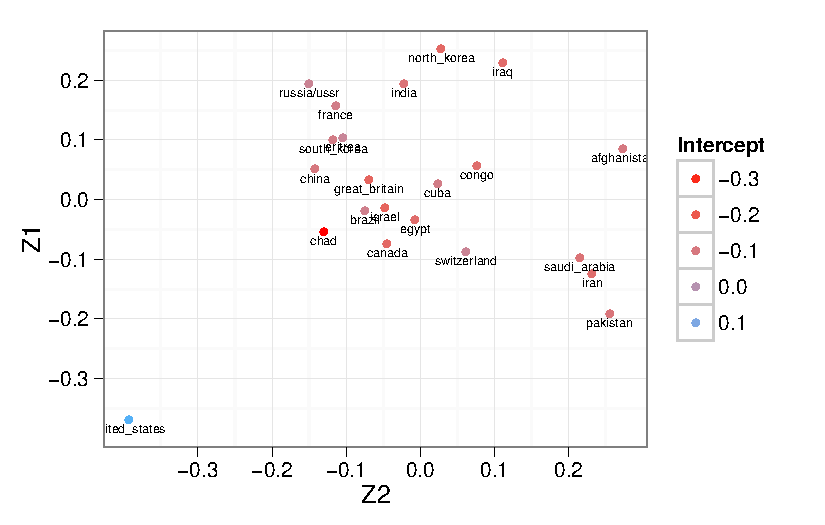
\includegraphics[width=0.5\textwidth]{chapter_foreign_relations/figures/011_static_positions_mturk.pdf} &
    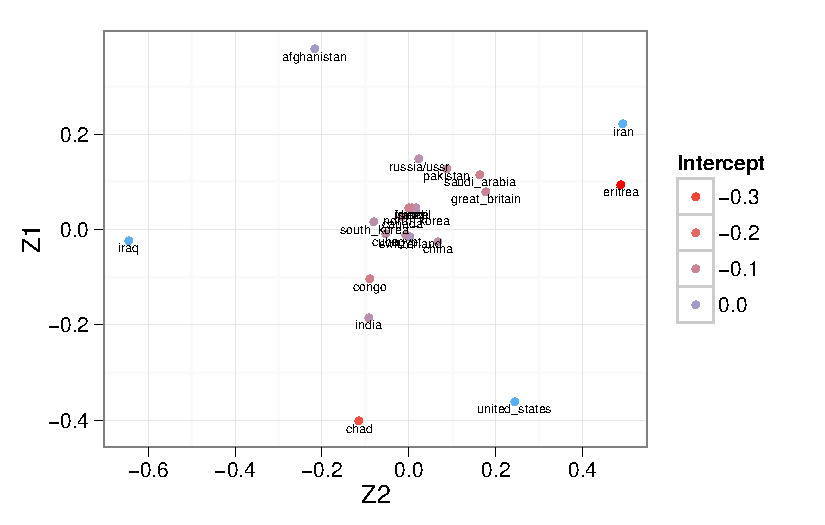
\includegraphics[width=0.5\textwidth]{chapter_foreign_relations/figures/011_static_positions_cow.pdf}
    \\
    Mechanical Turk & Correlates of War \\
  \end{tabular}
  \caption{Positions of selected countries according to the static
    issue-adjusted model for articles labeled with Amazon Mechanical
    Turk (left) and Correlates of War (right).  Countries' positions
    were inferred with the intercept / distance model, with distance
    dimension $p$=2.  Intercepts are illustrated by color.}
  \label{fig:fr_intercept_distance_positions}
\end{figure}

With both CoW and AMT labels, the relationships between
countries can be inferred from the distance between their positions.
In \myfig{fr_intercept_distance_positions}, the United States stands
out from a cluster of other countries, with Iraq, Iran, and
Afghanistan--countries with which the U.S. has been at odds in the past
twenty years--furthest away.

Correlates of War and Mechanical Turk labels provide different
patterns of inter-country sentiment.  Countries' positions under CoW
tend to be very clustered, with a few outliers, while their positions under
AMT labels are more uniformly distributed.  However, the two datasets
provide extraordinarily consistent measures of countries' relationships.

To measure the consistency of these two models, we measured the
Spearman rank correlation coefficient 
\begin{align*}
\underset{c_1, c_2 \in C, c_1   \neq c_2}
{\operatorname{\mbox{Correlation}}}(d_{\mbox{\tiny AMT}}(c_1, c_2), d_{\mbox{\tiny CoW}}(c_1, c_2))
\end{align*}
between all pairs of countries $c_1, c_2$ in the set $C$ of
countries. The two-dimensional \verb!intercept/distance! models have
a spearman rank correlation coefficient of $\sigma=0.900$.  Of course,
these $|C| \choose{2}$ distances are far from independent, and a
single outlier in each model could skew the correlation.  To mitigate
any such effect, we also measured the average correlation coefficient
\begin{align*}
  \frac{1}{|C|} \sum_{c_1 \in C}
  \underset{c_2 \in C, c_2 \neq c_1}
  {\operatorname{\mbox{Correlation}}}(d_{\mbox{\tiny AMT}}(c_i, c_2), d_{\mbox{\tiny
        CoW}}(c_i, c_2) ),
\end{align*}
which was \emph{even higher}, at $\sigma=0.901$. Recall that this is
higher than the correlation coefficient between the original labels
($\sigma=0.196$) -- an effect possible possible because these models
remove noise.

Under the second metric of correlation, most per-country correlations
were very high: over 90\% of countries had correlation coefficient
higher than 0.86.  One of the most-differently-represented countries
in this collection under the two different models was Iran, which
accounted for 7\% of documents; the per-Iran correlation coefficient
$\underset{c \in C, c \neq \mbox{\tiny Iran}}{\operatorname{\mbox{Cor}}}(d_{\mbox{\tiny AMT}}(\mbox{\small Iran}, c),
d_{\mbox{\tiny CoW}}(\mbox{\small Iran}, c)$ was 0.65 (higher only
than Eritrea, which was 0.62 but accounted for 0.2\% of documents).

\paragraph{Mutual sentiment with the United States and differences
 between CoW and AMT model fits.}
We illustrate mutual sentiment with the United states for a selection
of these countries over time in \myfig{country_positions_over_time}.
To estimate the sentiment in these plots, we fit the
\verb!intercept/distance! model with $\mbox{dim}(\bm z) = 2$.
We summarize major events for two of these countries below.
\begin{itemize}
  \item \textbf{Ukraine} was emancipated in 1991 with the dissolution
    of the Soviet Union.  The U.S. has given Ukraine over $4.1$
    billion in aid, targeted to ``promote political, security, and
    economic reform and to address urgent social and humanitarian
    needs'' \citep{ukrainestate:2012}.  In return, Ukrain has been an
    active member of the UN and has assisted the NATO allies with
    defense aid in Kosovo (1999), Afghanistan (2011), Iraq, the Middle
    East, and Africa.  Ukraine adopted its first post-Soviet
    constitution June 28, 1996, the same year taking part in the
    Olympics for the first time as an independent nation (the Olympics
    were hosted in the U.S. that year).  At the same time, Ukraine has
    been taking acrive steps in eliminating the nuclear weapons
    program it inherited, permanently closing the last operating
    reactor at the Chornobyl site in 2000 \citep{ukrainestate:2012}.

    Ukraine's sentiment with Iraq, as inferred from the AMT model, was
    at its lowest in January 1993, January 1998, and again in April
    2006.  Its CoW sentiment with Iraq was at its lowest in May 2006,
    April 2003, and February 1991 (technically before its
    independence, during the Persian Gulf War). Its relationship with
    the U.S. was much stronger than with Iraq, peaking in 1996 (AMT)
    and June 2002 (CoW), when it supported the U.S. invasion of Iraq.

  \item \textbf{Iran} has had a poor relationship with the United
    States since the U.S. Embassy seizure in 1981.  Between 1987 and
    1988, U.S. and Iranian forces clashed in the Persian Gulf.
    \citep{irancia:2012}.  Transfers of power have since then increased
    political tension, with the election of a reformist president in
    1997 and a reformist legislature in 2000, followed by conservative
    re-elections starting in 2003 and continuing through 2004.
    Hardliner President President Mahmud Ahmadinejad was inaugurated
    in August 2005 and re-elected in 2009 \citep{irancia:2012}.

    Ahmadinejad's rule has been met with increasing pressure from
    United Nations countries.  The Council has made successive
    resolutions imposing santions on Iran in 2006, 2007, 2008, and
    2010 \citep{iranstate:2012}.

    The Mechanical Turk sentiment between Iran and the U.S. has
    clearly dropped in the lead-up to Ahmadinejad's election (see
    again \myfig{country_positions_over_time}), but this contrasts
    with the Correlates of War sentiment, which was lowest in 1988,
    when AMT sentiment was not as low.

\end{itemize}
 
Both of these low periods with Iran are clearly periods of bad
relationships between these countries, but why did one model pick up
sentiment in one case and not the other?  This could be explained in
part because the tension picked up by the CoW labels was unilateral,
while the tension picked up in the later period did not fall under the
dictum of CoW labels: the U.S. and Iran were neither at war nor having
a territorial dispute.  Instead, the U.S., as a member of the U.N. has
supported Iran sanctions.


\begin{figure}
  \center
    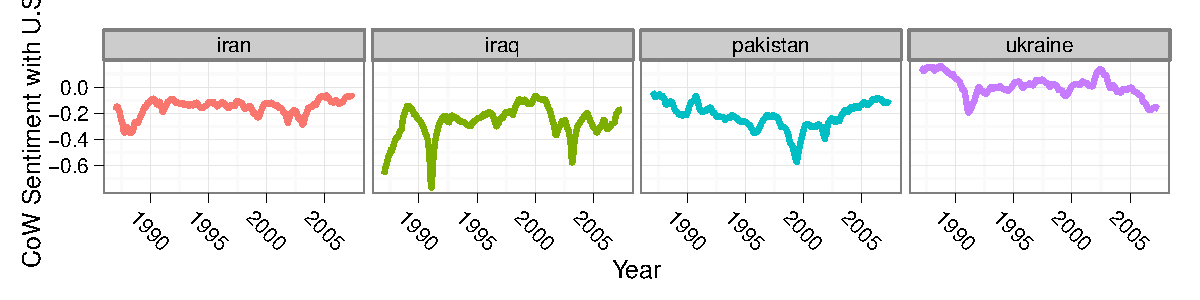
\includegraphics[width=1\textwidth]{chapter_foreign_relations/figures/012_fr_cow_mutual_sentiment_with_us.pdf}
    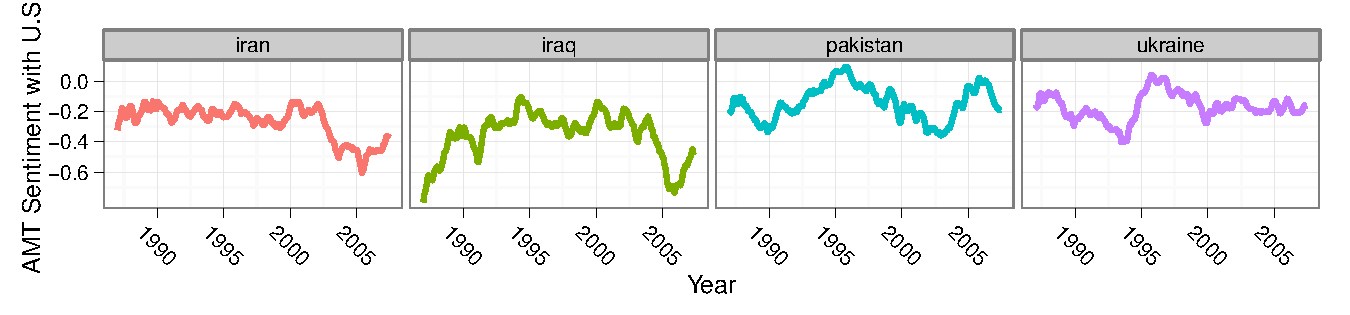
\includegraphics[width=1\textwidth]{chapter_foreign_relations/figures/012_fr_mturk_mutual_sentiment_with_us.pdf}
  \label{fig:country_positions_over_time}
  \caption{Selected countries' relationships with the United States
    over time.  Each line in the plot above represents a specific
    country's relationship with the United states inferred with the
    intercept/distance link function, with a two-dimensional distance
    space, using CoW labels (top) and AMT labels (bottom).  Sentiment
    between all countries and either Iran or Pakistan was
    least consistent between CoW and AMT. Ukraine was
    the most consistently represented with these labels.}
\end{figure}

% > a = read.csv("../../data/v4/v4-doc-training_samples.csv", as.is=TRUE, header=FALSE)

  %  We then evaluate perplexity
 % \begin{align}
 %   \mbox{perp}_d & = \mathcal{E_{\hat D}} \log p(w | \bar x_{d_{c1}}
 %     \bar x_{d_{c2}} ) \\
 %     & = \frac{1}{N} \sum_N \sum_{W_{d_n}}
 %     \log p(w | \bar x_{d_{c1}} \bar x_{d_{c2}} ) \\
 % \end{align}

% \subsubsection*{Bivariate change point detection}
% In addition to identifying the latent positions of nations over
% time, we can pinpoint periods of great change or upheaval.  Sudden
% changes in a nation's position is an indication of newsworthy events
% in its history; simultaneous changes in two nations' positions is an
% indication that they are both taking part in these newsworthy events.

% The task of identifying sudden changes in a time-series is known as
% change point detection.  Change point detection is frequently
% addressed by simple univariate significance tests.  We consider
% changes in the statistic $\bar s_{c1,c2} := \bar x_{c1} \bar x_{c2}$
% (see Equation~\ref{figure:sentiment}).  Because $\bar s_{c1,c1}$ may
% be change significantly when either $x_{c_1}$ or $x_{c_2}$ changes, we
% search for simultaneous significant changes in $\bar x_{c_1}$, $\bar
% x_{c_2}$, and $\bar s_{c1,c2}$ (Note that $\mathcal{E}[s_{c1,c2}] \neq
% \bar s_{c1,c2}$; we compute $\bar s_{c1,c2}$ out of convenience.

